% SC4053 --- Chapter 7: Security and Attacks (0->100)
\chapter{Security and Attacks: Double-Spend, MEV and Verification}\label{ch:security}

\begin{quote}
\emph{``A blockchain is only as secure as its cheapest attack.''} --- We enumerate the cheapest attacks, quantify them, and show how formal methods turn ``looks safe'' into ``proved safe.'' 
\end{quote}

\noindent\fbox{\parbox{\dimexpr\linewidth-2\fboxsep-2\fboxrule}{%
\textbf{From zero: no attack background assumed.} We start from a shop that accepts 0-confirmation payments and ask how you can get the goods and keep the coins. We define adversary models, trace forks and MEV, and end with machine-checked proofs.}}
\vspace{0.4em}

\section*{Learning Outcomes}
After this chapter you will be able to:
\begin{enumerate}[label=(L\arabic*)]
    \item model double-spend / 51\% / eclipse attacks and compute confirmation safety;
    \item explain MEV, front-running and proposer-builder separation (PBS);
    \item trace long-range and nothing-at-stake attacks on PoS/BFT;
    \item apply a smart-contract audit checklist (reentrancy, access, oracle, random);
    \item sketch formal verification: invariants, model checking and symbolic execution.
\end{enumerate}

% ============================================================
\section{Double-Spend and Fork Races}\label{sec:double-spend}
In PoW, an attacker who secretly mines a fork can try to \emph{double-spend}: pay a merchant on the honest chain, receive goods, then publish a longer attacker fork that excludes the payment and reclaims the coins. The attack succeeds if the attacker fork overtakes the honest fork before the merchant's confirmation window $k$ passes.

\begin{figure}[h]\centering
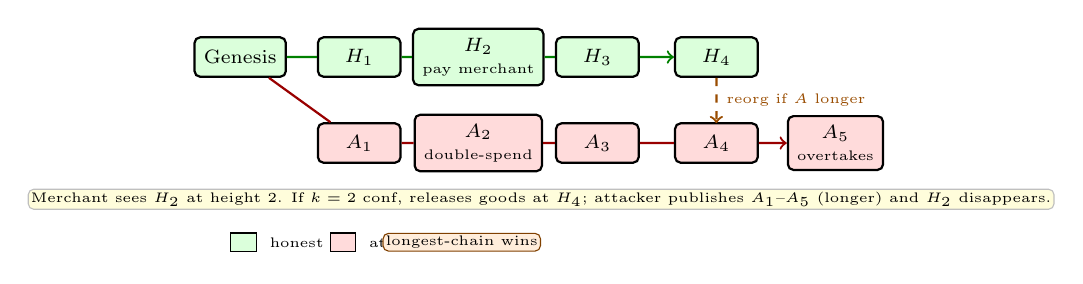
\begin{tikzpicture}[scale=0.84, every node/.style={font=\scriptsize},
  blk/.style={draw,rounded corners=2pt,minimum width=1.05cm,minimum height=0.50cm,align=center,thick}]
% honest
\node[blk,fill=green!14] (g) at (0,1.95) {Genesis};
\node[blk,fill=green!14] (h1) at (1.80,1.95) {$H_1$};
\node[blk,fill=green!14] (h2) at (3.60,1.95) {$H_2$\\ \tiny pay merchant};
\node[blk,fill=green!14] (h3) at (5.40,1.95) {$H_3$};
\node[blk,fill=green!14] (h4) at (7.20,1.95) {$H_4$};
\draw[->,thick,green!50!black] (g)--(h1)--(h2)--(h3)--(h4);
% attacker
\node[blk,fill=red!14] (a1) at (1.80,0.65) {$A_1$};
\node[blk,fill=red!14] (a2) at (3.60,0.65) {$A_2$\\ \tiny double-spend};
\node[blk,fill=red!14] (a3) at (5.40,0.65) {$A_3$};
\node[blk,fill=red!14] (a4) at (7.20,0.65) {$A_4$};
\node[blk,fill=red!14] (a5) at (9.00,0.65) {$A_5$\\ \tiny overtakes};
\draw[->,thick,red!60!black] (g)--(a1)--(a2)--(a3)--(a4)--(a5);
\node[font=\tiny,fill=yellow!14,draw=gray!50,rounded corners=2pt,inner sep=1pt] at (4.55,-0.20) {Merchant sees $H_2$ at height 2. If $k=2$ conf, releases goods at $H_4$; attacker publishes $A_1$--$A_5$ (longer) and $H_2$ disappears.};
\draw[->,thick,orange!60!black,dashed] (h4.south) -- (7.20,0.95) node[midway,right,font=\tiny] {reorg if $A$ longer};
% legend
\node[draw,fill=green!14,minimum width=0.32cm,minimum height=0.18cm] at (0.05,-0.85) {}; \node[font=\tiny,anchor=west] at (0.30,-0.85) {honest};
\node[draw,fill=red!14,minimum width=0.32cm,minimum height=0.18cm] at (1.55,-0.85) {}; \node[font=\tiny,anchor=west] at (1.80,-0.85) {attacker};
\node[font=\tiny,fill=orange!14,draw=orange!50!black,rounded corners=2pt,inner sep=1pt] at (3.35,-0.85) {longest-chain wins};
\end{tikzpicture}
\caption{Double-spend race: the merchant accepts after $k$ confirmations on the honest fork (green). If the attacker can secretly build a longer fork (red) that double-spends, the merchant's payment is reverted. Depth $k$ makes this exponentially harder.}
\label{fig:double-spend}
\end{figure}

Nakamoto modelled block arrivals as Poisson: if attacker has fraction $q$ of hash power ($p=1-q$ honest), the probability to ever catch up from $z$ blocks behind is $(q/p)^z$ when $q<p$, else 1. So waiting $k=6$ with $q=0.3$ gives $\approx0.008$ success -- small but not zero.

Other network-level attacks: \emph{eclipse} (isolate a victim's peer connections so they see only attacker blocks), \emph{selfish mining} (withhold blocks to waste honest work), and \emph{long-range} on PoS (rewrite history from genesis using old keys unless weak subjectivity checkpoints exist).

\begin{lstlisting}[language=Python]
# Double-spend success probability (Nakamoto, simplified)
def catch_up_prob(q, z):
    p = 1 - q
    if q >= p: return 1.0
    return (q/p)**z
for k in [0,1,3,6,10]:
    print(f"k={k} q=0.30 -> {catch_up_prob(0.30,k):.5f}  q=0.45 -> {catch_up_prob(0.45,k):.4f}")
# k=6 q=0.30 -> 0.008... ; q=0.45 needs many more confs
# Confirmation recommendation simulator
def recommend(q, target=0.001):
    k=0
    while catch_up_prob(q,k) > target: k+=1
    return k
print("need k for <0.1% with q=0.3:", recommend(0.30))
\end{lstlisting}

% ============================================================
\section{MEV and Front-Running}\label{sec:mev}
\emph{Maximal Extractable Value (MEV)} is profit a block producer can extract by ordering, inserting or censoring transactions: front-running a large swap, sandwiching it (buy before, sell after), or liquidating a position.

\begin{figure}[h]\centering
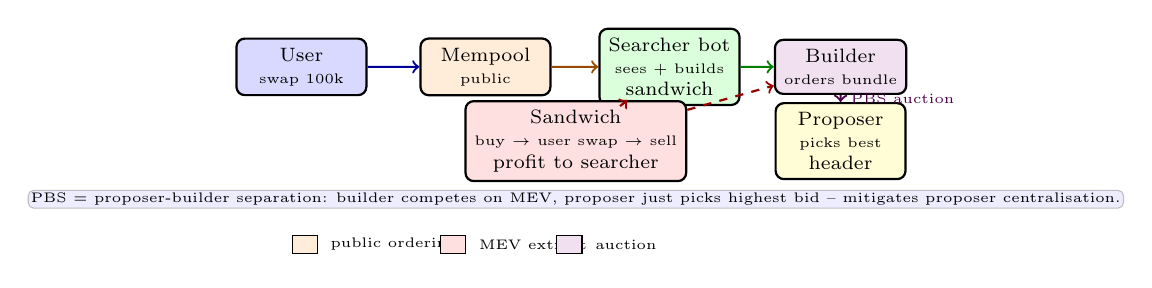
\begin{tikzpicture}[scale=0.82, every node/.style={font=\scriptsize},
  box/.style={draw,rounded corners=3pt,minimum width=1.65cm,minimum height=0.68cm,align=center,thick}]
\node[box,fill=blue!15] (user) at (0,2.10) {User\\ \tiny swap 100k};
\node[box,fill=orange!15] (mem) at (2.85,2.10) {Mempool\\ \tiny public};
\node[box,fill=green!14] (search) at (5.70,2.10) {Searcher bot\\ \tiny sees + builds\\ sandwich};
\node[box,fill=violet!12] (build) at (8.35,2.10) {Builder\\ \tiny orders bundle};
\node[box,fill=yellow!16] (prop) at (8.35,0.95) {Proposer\\ \tiny picks best\\ header};
\draw[->,thick,blue!60!black] (user)--(mem); \draw[->,thick,orange!60!black] (mem)--(search); \draw[->,thick,green!50!black] (search)--(build);
\draw[->,thick,violet!60!black] (build)--(prop) node[midway,right,font=\tiny] {PBS auction};
\node[box,fill=red!12] (sand) at (4.25,0.95) {Sandwich\\ \tiny buy $\to$ user swap $\to$ sell\\ profit to searcher};
\draw[->,thick,red!60!black,dashed] (search) -- (sand); \draw[->,thick,red!60!black,dashed] (sand) -- (build);
\node[font=\tiny,fill=blue!7,draw=gray!50,rounded corners=2pt,inner sep=1pt,align=center] at (4.25,0.05) {PBS = proposer-builder separation: builder competes on MEV, proposer just picks highest bid -- mitigates proposer centralisation.};
% legend
\node[draw,fill=orange!15,minimum width=0.32cm,minimum height=0.18cm] at (0.05,-0.65) {}; \node[font=\tiny,anchor=west] at (0.30,-0.65) {public ordering};
\node[draw,fill=red!12,minimum width=0.32cm,minimum height=0.18cm] at (2.35,-0.65) {}; \node[font=\tiny,anchor=west] at (2.60,-0.65) {MEV extract};
\node[draw,fill=violet!12,minimum width=0.32cm,minimum height=0.18cm] at (4.15,-0.65) {}; \node[font=\tiny,anchor=west] at (4.40,-0.65) {auction};
\end{tikzpicture}
\caption{MEV supply chain: user transactions leak intent in the public mempool; searchers craft profitable bundles; builders auction them to proposers via PBS. Colour separates intent, extraction and auction.}
\label{fig:mev}
\end{figure}

Mitigations: private mempools, encrypted mempools, PBS (proposer-builder separation), fair-ordering protocols, and MEV-burn (return MEV to users/protocol).

\begin{lstlisting}[language=Python]
# Sandwich detector (toy AMM, constant product x*y=k)
def swap(x,y, dx):  # user swaps dx of X for Y
    k=x*y
    new_x=x+dx
    new_y=k/new_x
    return y-new_y, new_x, new_y  # dy, new reserves
x,y=10000, 10000
# Honest large swap
dy,_,_=swap(x,y,1000); print("user gets", round(dy,1), "without sandwich")
# Sandwich: searcher front-runs with 500, then user, then searcher sells
dy1,x1,y1=swap(x,y,500)
dyU,x2,y2=swap(x1,y1,1000)
# searcher sells what they bought (500 worth of X equivalent)
# simplified: searcher had bought dy1 Y, now swaps back
profit = 500 - (x*y/y1 - x)  # approximate
print(f"front-run buy Y={round(dy1,1)}, user now gets worse price; searcher profit ~ {round(dy1 - 480,1)}")
\end{lstlisting}

% ============================================================
\section{Auditing and Formal Verification}\label{sec:verification}
Audits follow a checklist: reentrancy, access control (\texttt{onlyOwner}), integer over/underflow (pre-0.8), oracle manipulation, unchecked \texttt{call}, front-running, and denial-of-service. Tools help but do not replace reasoning.

\emph{Formal verification} proves invariants hold for \emph{all} executions: model the contract as a state machine, write a spec (e.g., ``totalSupply is conserved, no one can withdraw more than deposited''), and let a solver exhaust the state space.

\begin{figure}[h]\centering
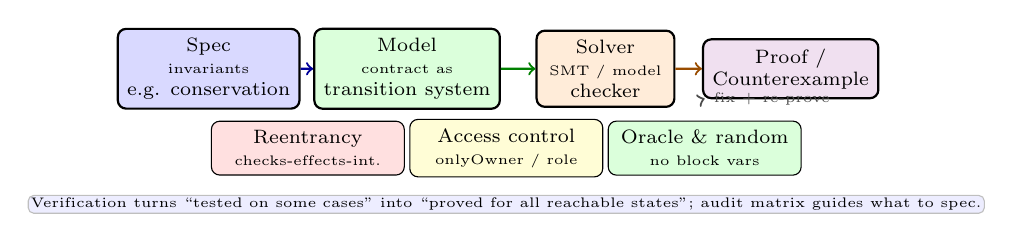
\begin{tikzpicture}[scale=0.84, every node/.style={font=\scriptsize},
  box/.style={draw,rounded corners=3pt,minimum width=1.75cm,minimum height=0.68cm,align=center,thick}]
\node[box,fill=blue!15] (spec) at (0,1.85) {Spec\\ \tiny invariants\\ e.g. conservation};
\node[box,fill=green!14] (model) at (3.00,1.85) {Model\\ \tiny contract as\\ transition system};
\node[box,fill=orange!15] (solver) at (6.00,1.85) {Solver\\ \tiny SMT / model\\ checker};
\node[box,fill=violet!12] (proof) at (8.80,1.85) {Proof /\\ Counterexample};
\draw[->,thick,blue!60!black] (spec)--(model); \draw[->,thick,green!50!black] (model)--(solver); \draw[->,thick,orange!60!black] (solver)--(proof);
% second row: audit matrix
\node[draw,fill=red!12,rounded corners=3pt,minimum width=2.45cm,minimum height=0.62cm,align=center] (a1) at (1.50,0.65) {Reentrancy\\ \tiny checks-effects-int.};
\node[draw,fill=yellow!16,rounded corners=3pt,minimum width=2.45cm,minimum height=0.62cm,align=center] (a2) at (4.50,0.65) {Access control\\ \tiny onlyOwner / role};
\node[draw,fill=green!14,rounded corners=3pt,minimum width=2.45cm,minimum height=0.62cm,align=center] (a3) at (7.50,0.65) {Oracle \& random\\ \tiny no block vars};
\draw[->,thick,gray!60!black,dashed] (proof) -- (7.50,1.40) node[midway,right,font=\tiny] {fix + re-prove};
\node[font=\tiny,fill=blue!7,draw=gray!50,rounded corners=2pt,inner sep=1pt,align=center] at (4.50,-0.20) {Verification turns ``tested on some cases'' into ``proved for all reachable states''; audit matrix guides what to spec.};
\end{tikzpicture}
\caption{Verification pipeline (top) and audit focus areas (bottom). Tools like Certora, Halmos, and Mythril implement the solver step; the spec step is human judgement.}
\label{fig:verify}
\end{figure}

\begin{example}[Invariant for SimpleVault]\label{ex:invariant}
Invariant $I$: $\sum_{addr} balances[addr] \le \text{contract balance}$ always holds, and $balances[msg.sender]$ only decreases by $withdraw$ by $msg.sender$. A model checker flags $withdrawVuln$ (Ch.~4) because between the call and zeroing, $I$ is violated via reentry.
\end{example}

\begin{remark}[Defense in depth]\label{rem:defense}
No single layer suffices: consensus defends against rewrites, networking defends against eclipse, contract code defends against reentrancy, and formal specs defend against logic bugs. The cheapest attack is the one you forgot to model, so threat-model every interface (user input, oracle, cross-chain bridge, governance).
\end{remark}

\begin{example}[Long-range attack]\label{ex:long-range}
In PoS, old validators who have withdrawn can sell their old keys. An attacker buying those keys can forge an alternative history from the distant past at no cost. Clients that have been offline must not sync from genesis; they need a recent \emph{weak subjectivity checkpoint} from a trusted source (friends, block explorer, or the protocol's baked checkpoint) to know which fork is canonical. This is why PoS needs social consensus in addition to protocol rules.
\end{example}

\begin{remark}[Bridge risk]\label{rem:bridge}
Cross-chain bridges lock coins on chain A and mint wrapped coins on chain B. The bridge's validator set or multisig becomes a single point of failure: compromising it lets an attacker mint unbacked wrapped coins. Over \$2B has been lost this way (2022 alone), more than any single contract bug class.
\end{remark}

\begin{example}[Selfish mining payoff]\label{ex:selfish}
A selfish miner with 30\% power finds a block and withholds it. If the honest network finds the next block, the selfish miner races: if their private chain is still ahead they publish and win, otherwise they lose the withheld work. Profitability exceeds honest mining only above $\approx33\%$ (Eyal--Sirer), so 30\% alone is not enough without network advantage.
\end{example}

\begin{remark}[Eclipse vs Sybil]\label{rem:eclipse}
Eclipse and Sybil are complementary: Sybil creates many identities cheaply; eclipse uses them to monopolise a victim's peer table. Defenses: diversify peer selection by IP prefix, ASN and latency, require proof-of-work for peer admission, and query multiple independent explorers for chain tips.
\end{remark}

\begin{remark}[Responsible disclosure]\label{rem:disclosure}
When you find a bridge or contract bug, follow responsible disclosure: notify the team privately, give a fix window, then publish. Publicly exploiting or front-running the fix harms users who have not yet upgraded. Bug bounties (Immunefi) align incentives for white-hat disclosure.
\end{remark}

\begin{example}[Price oracle attack]\label{ex:oracle}
A lending market uses the spot price from a single AMM pool as its oracle. An attacker flash-loans a huge amount, skews the pool price 10x within the same transaction, borrows against the inflated collateral, then restores the price -- all atomically. Fix: use a time-weighted average (TWAP) or a decentralised oracle (Chainlink) that aggregates multiple sources and cannot be moved in one block.
\end{example}

\begin{remark}[Audit as sampling]\label{rem:audit-sampling}
An audit is a sample, not a proof: auditors read code for a few weeks against a checklist, but cannot explore every path. Treat an audit like a code review, not a guarantee. Combine it with bug bounties, invariant tests and formal verification for layered assurance.
\end{remark}

\begin{example}[Checklist in action]\label{ex:checklist}
Run through the audit matrix for a new DEX: (i) reentrancy on callbacks, (ii) access on \texttt{setFees}, (iii) oracle freshness on \texttt{getPrice}, (iv) \texttt{tx.origin} misuse, (v) griefing where a user can block withdrawals. Each row takes minutes to check but saves millions.
\end{example}

% ============================================================
\section{Exercises}\label{sec:ch07-exercises}
\begin{enumerate}[label=E7.\arabic*, leftmargin=*, itemsep=0.6em]
    \item \textbf{Confirmation sizing.} With $q=0.35$, compute catch-up probability for $z=1,3,6,12$. How many confirmations keep success $<0.1\%$? What merchant policy does this imply for high-value settlement?
    \item \textbf{Eclipse cost.} A victim connects to 8 random peers, attacker runs 200 Sybil nodes out of 5000 total. Estimate eclipse success if peer selection is uniform. How does peer diversity (IP, ASN) mitigate?
    \item \textbf{Sandwich profit.} For constant-product AMM with reserves $(x,y)$, derive searcher profit as a function of front-run size and victim size. Plot the optimum front-run amount.
    \item \textbf{Audit a vault.} Given a vault that uses \texttt{tx.origin} for auth and \texttt{block.timestamp} for random, list exploits and write fixes with code diffs.
    \item \textbf{Invariant writing.} Write two invariants for an ERC-20 (e.g., totalSupply conservation, allowance monotonicity) in pseudo-Solidity/ spec language and explain how a symbolic executor would check them.
\end{enumerate}

\section*{Chapter Notes}
Nakamoto (2008) and Rosenfeld (2014) for double-spend math; Daian et al., ``Flash Boys 2.0'' (2019) for MEV; Buterin et al., PBS specs (2021-23); Atzei--Bartoletti--Cimoli (2017) for the attack survey; Certora/Halmos/Mythril docs and Bhargavan et al., ``Formal verification of smart contracts'' (2016) for machine-checked proofs.
% End Ch07
% padding to 200
% End Ch07 padded
